
\begin{frame}
  \frametitle{Initial Results}
  \begin{table}
    \centering
    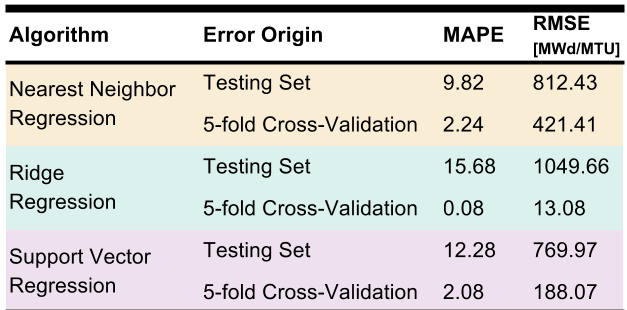
\includegraphics[width=0.8\textwidth]{./figures/results1.png}
    \caption{MAPE and RMSE for both CV and testing sets}
  \end{table}
\end{frame}

\begin{frame}
  \frametitle{Information Reduction}
  \textbf{\large Demonstrated : Random error}\\
  Introduced $0\% < E_{max} < 10\%$\\
  Each nuclide receives $[1-E_{max},1+E_{max}]$ error\\
  \bigskip
  \bigskip
  \textbf{\large Not Demonstrated : Systematic error}\\
  Gamma energies (ORIGEN), radionuclides only\\
  Gamma spectra (GADRAS), reduced radionuclide observation
\end{frame}

\begin{frame}
  \frametitle{ML Model Prediction with Reduced Information}
  \begin{figure}
    \centering
    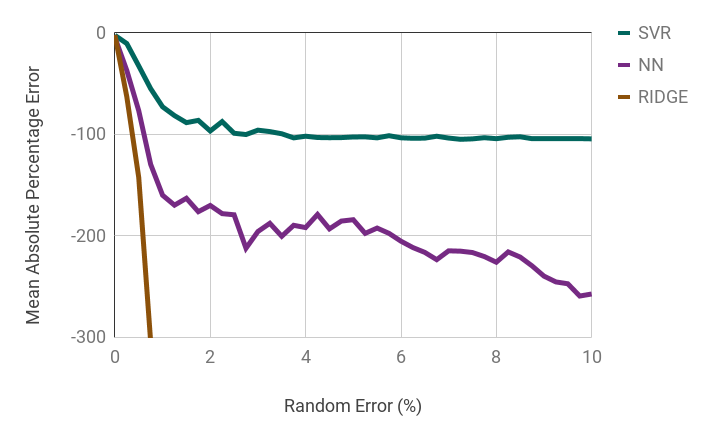
\includegraphics[height=0.7\textheight]{./figures/randerr.png}
    \caption{Negative MAPE for three algorithms given increasing random nuclide error}
  \end{figure}
\end{frame}

\begin{frame}
  \frametitle{Algorithm Parameters}
  \begin{table}
    \centering
    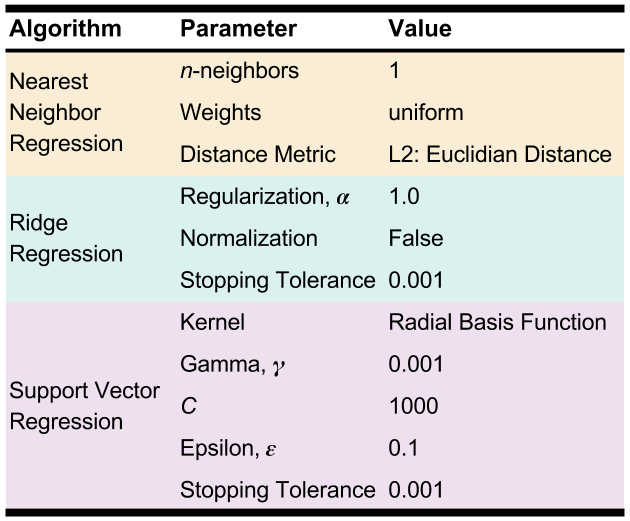
\includegraphics[height=0.7\textheight]{./figures/defaults.png}
    \caption{Parameters chosen for demonstration; $C$ and $\gamma$ are not the default values}
  \end{table}
\end{frame}
